\documentclass[letterpaper]{article} % DO NOT CHANGE THIS
\usepackage{aaai2027}  % DO NOT CHANGE THIS
\usepackage[hyphens]{url}  % DO NOT CHANGE THIS
\usepackage{graphicx} % DO NOT CHANGE THIS
\urlstyle{rm} % DO NOT CHANGE THIS
\def\UrlFont{\rm}  % DO NOT CHANGE THIS
\usepackage{natbib}  % DO NOT CHANGE THIS AND DO NOT ADD ANY OPTIONS TO IT
\InputIfFileExists{early-cites.tex}{}{\bibcite{asai2024selfrag}{{1}{2024}{{Asai et~al.}}{{Asai, Wu, Wang, Sil, and Hajishirzi}}}
\bibcite{borgeaud2022retro}{{2}{2021}{{Borgeaud et~al.}}{{Borgeaud, Mensch, Hoffmann, Cai, Rutherford, Millican, van den Driessche, Lespiau, Damoc, Clark, de Las Casas, Guy, Menick, Ring, Hennigan, Huang, Maggiore, Jones, Cassirer, Brock, Paganini, Irving, Vinyals, Osindero, Simonyan, Rae, Elsen, and Sifre}}}
\bibcite{chen2023frugalgpt}{{3}{2023}{{Chen et~al.}}{{Chen, Zaharia, and Zou}}}
\bibcite{chen2025research}{{4}{2025}{{Chen et~al.}}{{Chen, Sun, Li, Sun, Zhou, Zhu, Wang, Pan, Zhang, Chen, Yang, Zhou, and Chen}}}
\bibcite{gandhi2026grasp}{{5}{2026}{{Gandhi et~al.}}{{Gandhi, Lee, Todmal, Dernoncourt, Rossi, Wang, and Lan}}}
\bibcite{gao2023rarr}{{6}{2022}{{Gao et~al.}}{{Gao, Dai, Pasupat, Chen, Chaganty, Fan, Zhao, Lao, Lee, Juan, and Guu}}}
\bibcite{gao2023hyde}{{7}{2022}{{Gao et~al.}}{{Gao, Ma, Lin, and Callan}}}
\bibcite{gao2022tevatron}{{8}{2022}{{Gao et~al.}}{{Gao, Ma, Lin, and Callan}}}
\bibcite{guu2020realm}{{9}{2020}{{Guu et~al.}}{{Guu, Lee, Tung, Pasupat, and Chang}}}
\bibcite{honovich2022true}{{10}{2022}{{Honovich et~al.}}{{Honovich, Aharoni, Herzig, Taitelbaum, Kukliansy, Cohen, Scialom, Szpektor, Hassidim, and Matias}}}
\bibcite{izacard2021fid}{{11}{2020}{{Izacard and Grave}}{{}}}
\bibcite{izacard2023atlas}{{12}{2022}{{Izacard et~al.}}{{Izacard, Lewis, Lomeli, Hosseini, Petroni, Schick, Dwivedi-Yu, Joulin, Riedel, and Grave}}}
\bibcite{jeong2024adaptive}{{13}{2024}{{Jeong et~al.}}{{Jeong, Baek, Cho, Hwang, and Park}}}
\bibcite{jiang2023flare}{{14}{2023}{{Jiang et~al.}}{{Jiang, Xu, Gao, Sun, Liu, Dwivedi-Yu, Yang, Callan, and Neubig}}}
\bibcite{jin2025searchr1}{{15}{2025}{{Jin et~al.}}{{Jin, Zeng, Yue, Yoon, Arik, Wang, Zamani, and Han}}}
\bibcite{karpukhin2020dpr}{{16}{2020}{{Karpukhin et~al.}}{{Karpukhin, O{\u{g}}uz, Min, Lewis, Wu, Edunov, Chen, and Yih}}}
\bibcite{kwiatkowski2019nq}{{17}{2019}{{Kwiatkowski et~al.}}{{Kwiatkowski, Palomaki, Redfield, Collins, Parikh, Alberti, Epstein, Polosukhin, Devlin, Lee, Toutanova, Jones, Kelcey, Chang, Dai, Uszkoreit, Le, and Petrov}}}
\bibcite{lewis2020rag}{{18}{2020}{{Lewis et~al.}}{{Lewis, Perez, Piktus, Petroni, Karpukhin, Goyal, K{\"u}ttler, Lewis, Yih, Rockt{\"a}schel, Riedel, and Kiela}}}
\bibcite{ma2023rewrite}{{19}{2023}{{Ma et~al.}}{{Ma, Gong, He, Zhao, and Duan}}}
\bibcite{nogueira2019monobert}{{20}{2019}{{Nogueira and Cho}}{{}}}
\bibcite{ong2024routellm}{{21}{2024}{{Ong et~al.}}{{Ong, Almahairi, Wu, Chiang, Wu, Gonzalez, Kadous, and Stoica}}}
\bibcite{press2023selfask}{{22}{2022}{{Press et~al.}}{{Press, Zhang, Min, Schmidt, Smith, and Lewis}}}
\bibcite{qwen2024}{{23}{2024}{{Qwen Team}}{{}}}
\bibcite{rajpurkar2016squad}{{24}{2016}{{Rajpurkar et~al.}}{{Rajpurkar, Zhang, Lopyrev, and Liang}}}
\bibcite{robertson2009bm25}{{25}{2009}{{Robertson and Zaragoza}}{{}}}
\bibcite{schick2023toolformer}{{26}{2023}{{Schick et~al.}}{{Schick, Dwivedi-Yu, Dess{\`i}, Raileanu, Lomeli, Zettlemoyer, Cancedda, and Scialom}}}
\bibcite{schulman2017ppo}{{27}{2017}{{Schulman et~al.}}{{Schulman, Wolski, Dhariwal, Radford, and Klimov}}}
\bibcite{shao2024deepseekmath}{{28}{2024}{{Shao et~al.}}{{Shao, Wang, Zhu, Xu, Song, Bi, Zhang, Zhang, Li, Wu, and Guo}}}
\bibcite{song2025r1searcher}{{29}{2025}{{Song et~al.}}{{Song, Jiang, Min, Chen, Chen, Zhao, Fang, and Wen}}}
\bibcite{su2024dragin}{{30}{2024}{{Su et~al.}}{{Su, Tang, Ai, Wu, and Liu}}}
\bibcite{sun2023rankgpt}{{31}{2023}{{Sun et~al.}}{{Sun, Yan, Ma, Wang, Ren, Chen, Yin, and Ren}}}
\bibcite{trivedi2023ircot}{{32}{2022}{{Trivedi et~al.}}{{Trivedi, Balasubramanian, Khot, and Sabharwal}}}
\bibcite{williams1992reinforce}{{33}{1992}{{Williams}}{{}}}
\bibcite{yan2024crag}{{34}{2024}{{Yan et~al.}}{{Yan, Gu, Zhu, and Ling}}}
\bibcite{yang2018hotpotqa}{{35}{2018}{{Yang et~al.}}{{Yang, Qi, Zhang, Bengio, Cohen, Salakhutdinov, and Manning}}}
\bibcite{yao2023react}{{36}{2023}{{Yao et~al.}}{{Yao, Zhao, Yu, Du, Shafran, Narasimhan, and Cao}}}
}
\usepackage{caption} % DO NOT CHANGE THIS AND DO NOT ADD ANY OPTIONS TO IT
\frenchspacing  % DO NOT CHANGE THIS
\usepackage{amsmath}
\usepackage{booktabs}
\pdfinfo{
/TemplateVersion (2027.1)
}

\setcounter{secnumdepth}{1}

\title{Cost-Aware Reinforcement Learning for Agentic RAG}
\author{Parsuram Pradhan}
\affiliations{}

\begin{document}

\maketitle

\begin{abstract}
Tools help on some questions and hurt on others, so the average can stay flat. We price retrieve, rewrite, rerank, verify, and stop inside one retrieval episode, and we train a 357-parameter controller with REINFORCE. The reward subtracts token dollars, retrieval dollars, a fixed latency table, and a charge per action from answer quality. On 150 HotpotQA items and 150 Natural Questions items, with BM25 over 83{,}120 passages, one-shot retrieval scores 60/150 and 40/150. Max tools scores 62/150 and 43/150. That is 105 correct against 100, and the reward falls from 0.581 to 0.503. Three seeds at dollar weight 20 each select rewrite, then rewrite, then retrieve, then stop. The recipe scores 52/150 and 48/150, again 100 correct. It repairs 5 HotpotQA answers and breaks 13, and repairs 17 Natural Questions answers and breaks 9. The union is 122. The branch on retrieval strength appears in 0 of 3 seeds.
\end{abstract}

\section{Introduction}
On the Natural Questions item ``what is the name of wonder womans mother,'' one-shot retrieval returns passages titled Seoul Korea Temple and Flash in other media, and the generator answers Stevie Wonder. Two rewrites, together \(2.4\times 10^{-5}\) dollars, change the query to ``mother of wonder woman.'' The next search returns Wonder Girl and Duke of Deception, and the answer is Queen Hippolyta. The episode costs \(2.06\times 10^{-4}\) dollars, against \(1.83\times 10^{-4}\) for one-shot retrieval. On this question the rewrite pays. On others it does not.

That is the story. Tools help per question, not on average. The reward decides which tools survive. A small controller can lock onto one recipe and still miss the per-question choice.

Figure~\ref{fig:pipeline} is the whole pipeline. The generator and the retriever are frozen. Every number below is on one index of 83{,}120 passages.
\begin{itemize}
\item The reward decides which tools survive. Max tools scores 62/150 on HotpotQA and 43/150 on Natural Questions, against 60/150 and 40/150 for one-shot retrieval. Five more answers, and the reward falls from 0.581 to 0.503, because the action charge rises by 0.10 and the weighted quality terms rise by about 0.025.
\item The help is per question. The learned recipe and one-shot retrieval each score 100/300. The recipe is 52/150 and 48/150. One-shot retrieval is 60/150 and 40/150. The recipe repairs 5 HotpotQA answers and breaks 13, and repairs 17 Natural Questions answers and breaks 9. The union is 122/300. An oracle over one-shot retrieval, a six-step recipe, and max tools, keeping the cheapest correct trajectory, scores 107/300 at \(1.85\times 10^{-4}\) dollars. The six-step recipe adds no question one-shot retrieval missed.
\item The controller finds a stable recipe and does not learn that choice. Seeds 42, 43, and 44 at \(\lambda{=}20\) each emit rewrite, rewrite, retrieve, stop on all 300 questions. The second action still sees a retrieval score of 0. The branch on retrieval strength appears in 0 of 3 seeds.
\end{itemize}

\section{Related Work}
Retrieval-augmented generation conditions a generator on retrieved text \cite{lewis2020rag}. Agentic controllers interleave that retrieval with other tools. ReAct alternates reasoning traces and actions \cite{yao2023react}. The five systems in Table~\ref{tab:related} are the ones a reader will set this paper against. Each decides something about retrieval. None prices rewrite, rerank, and verify in dollars inside a closed loop.

\begin{table*}[t]
\centering
\small
\setlength{\tabcolsep}{4pt}
\begin{tabular}{lp{3.6cm}p{3.4cm}p{4.6cm}}
\toprule
Method & What it decides & What it prices & What we add \\
\midrule
Adaptive-RAG \cite{jeong2024adaptive} &
No retrieval, one retrieval, or multi-step retrieval, from the question alone &
Step count and relative time &
A second look after the passages arrive, with dollars and a per-action charge \\
Self-RAG \cite{asai2024selfrag} &
Whether to retrieve, and whether a segment is supported, as tokens in the generator &
Hand-set critique weights &
A frozen generator. Critique is one typed action with a measured cost \\
CRAG \cite{yan2024crag} &
Keep, discard, or mix the retrieved set. Discard triggers a web search &
An evaluator threshold &
Rewrite, rerank, and verify on a closed corpus \\
Search-R1 \cite{jin2025searchr1} &
When the language model itself emits a search during reasoning &
Answer correctness &
A small controller, so a change in exact match is a change in control \\
GRASP \cite{gandhi2026grasp} &
Semantic search, keyword search, or a paragraph read &
Answer quality, grounded reading, using both searches, and a turn count &
Rewrite, rerank, and verify, priced in dollars \\
\bottomrule
\end{tabular}
\caption{Published controllers this paper is positioned against. None is reimplemented on this stack. Adaptive-RAG is the row that could be: it is a classifier in front of no retrieval, one-shot retrieval, and a capped multi-step loop, all of which this environment already runs. That classifier is not trained here, so Adaptive-RAG is not a row in the results.}
\label{tab:related}
\end{table*}

Search-R1 trains the language model with an outcome reward to issue searches and reason over the results \cite{jin2025searchr1}. GRASP is the closest typed-action neighbor: a GRPO policy over semantic search, keyword search, and paragraph reading, rewarded for answer F1, grounded reading, complementary search, and turn efficiency \cite{gandhi2026grasp}. The efficiency term is paid only when answer F1 exceeds 0.5, and it counts turns, not dollars. GRASP does not price rewrite, rerank, or verification. We keep the generator fixed and ask a prior question: once those tools have a dollar cost, does a learned controller spend them only when they pay?

\mbox{FrugalGPT} and \mbox{RouteLLM} price a different choice. \mbox{FrugalGPT} cascades queries across LLM APIs whose fees differ by orders of magnitude, so a cheap model answers when it can and an expensive model answers when it must \cite{chen2023frugalgpt}. \mbox{RouteLLM} learns a router from preference data and sends each query to a strong model or a weak one \cite{ong2024routellm}. Both decide which model to call. We use one generator, Qwen2.5-3B-Instruct, and price the tool calls inside the episode.

The retrieval line behind that \mbox{generator} is older than the agent. REALM trains a retriever inside language-model pretraining \cite{guu2020realm}. Fusion-in-Decoder reads each retrieved passage on its own and fuses them in the decoder \cite{izacard2021fid}. RETRO conditions each chunk of the generation on neighbors from a trillion-token store \cite{borgeaud2022retro}. Atlas asks how far a retrieval-augmented model can go in the few-shot regime \cite{izacard2023atlas}.

Later controllers decide when to search again. IRCoT interleaves retrieval with chain-of-thought steps \cite{trivedi2023ircot}. FLARE retrieves when the next sentence looks uncertain \cite{jiang2023flare}. DRAGIN triggers retrieval from the model's own information need \cite{su2024dragin}. Self-Ask splits a multi-hop question into follow-ups \cite{press2023selfask}. Toolformer inserts API calls, including a search engine, into the generation \cite{schick2023toolformer}. On the query side, Ma et al.\ rewrite, then retrieve, then read \cite{ma2023rewrite}. HyDE embeds a hypothetical answering passage instead of the question \cite{gao2023hyde}. monoBERT reranks BM25 hits with a cross-encoder \cite{nogueira2019monobert}. RankGPT asks a language model to permute the candidates \cite{sun2023rankgpt}.

The training line splits the same way. PPO is the usual clipped policy gradient \cite{schulman2017ppo}. GRPO, introduced for math reasoning, replaces the learned critic with a group of rollouts of the same prompt \cite{shao2024deepseekmath}. R1-Searcher and ReSearch use that style of update to teach a language model to search \cite{song2025r1searcher,chen2025research}. RARR looks up evidence and revises a statement that the evidence does not support \cite{gao2023rarr}. TRUE compares the metrics people use for that kind of check \cite{honovich2022true}. We do not reimplement these systems. They are the decisions our five actions stand in for.

\section{Method}
Figure~\ref{fig:pipeline} is the protocol. An episode is one question. The controller picks one action at each step. The episode ends at stop, or when the step or budget cap forces a stop.

\begin{figure*}[t]
\centering
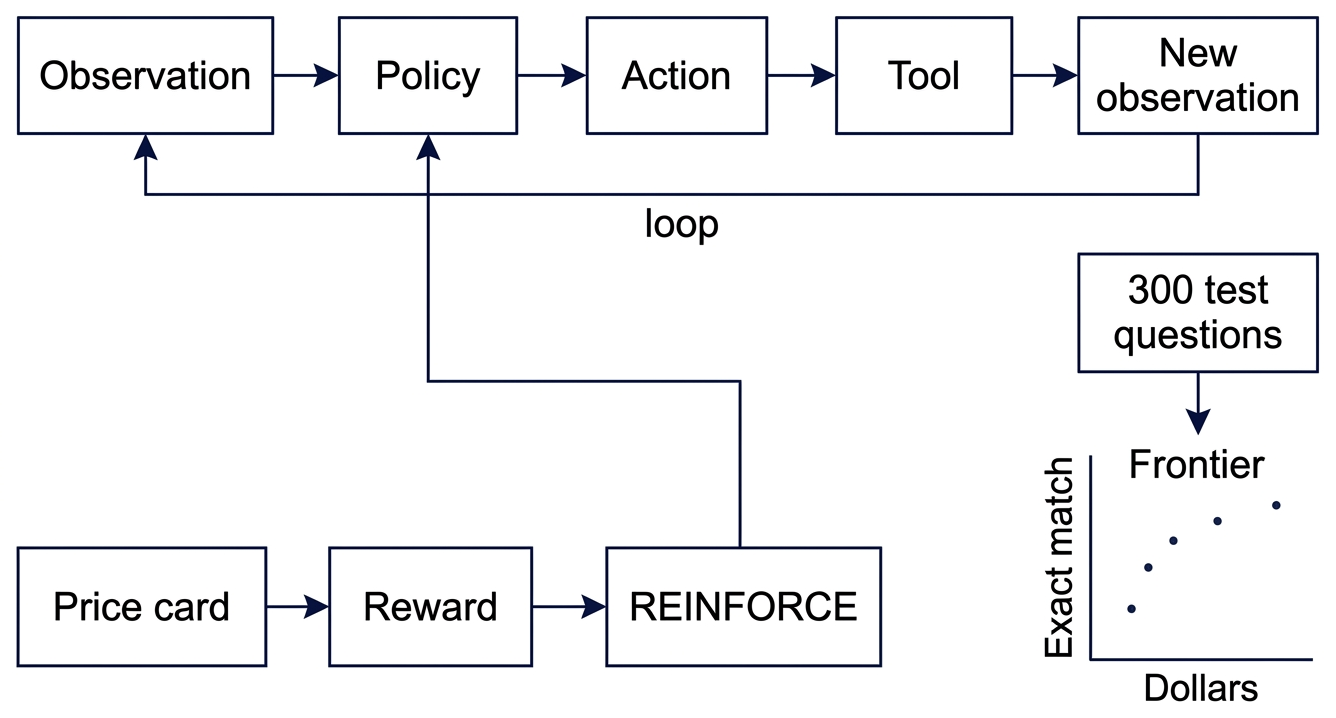
\includegraphics[width=\textwidth]{paper_v4/figures/pipeline.png}
\caption{The pipeline, as drawn. The top row loops from observation to the policy, an action, a tool, and a new observation. The price card feeds the reward, and REINFORCE carries that reward back to the policy. The 300 test questions feed the frontier, exact match against dollars.}
\label{fig:pipeline}
\end{figure*}

\subsection{Actions, Retriever, and Generator}
The action set is retrieve, rewrite, rerank, verify, and stop. Retrieve runs BM25 \cite{robertson2009bm25} and appends the top five passages. Rewrite asks the generator for a new query. Rerank reorders the current pool by lexical overlap with the query. Verify runs a lexical natural-language-inference check of the current draft and returns support, neutral, or contradiction. Stop emits a short answer, or abstains. Yes/no questions must be answered yes or no. Caps are eight steps, three retrieves, two rewrites, two reranks, and two verifies. Illegal actions are masked: with no evidence the policy cannot rerank, verify, or stop.

The generator is Qwen2.5-3B-Instruct at temperature 0 \cite{qwen2024}. Decoding is greedy. It reads the passages. The controller does not. The verifier is lexical, not a cross-encoder and not the generator judging itself. Training ran on one NVIDIA T4. The policy itself is a CPU network.

The price card meters local tokens at \$0.15 and \$0.60 per million input and output tokens, and BM25 at \(5\times 10^{-5}\) dollars per call. Latency in the reward and in the budget check is a fixed table, not the wall clock: 212.4 ms per retrieve, 999.2 ms per rewrite, 143.2 ms per rerank, 0 ms per verify, and 853.9 ms plus 52.0 ms per completion token for a generation. Those values are the median measured cost of the same calls, so the term keeps its size. A wall-clock charge would make two episodes with the same actions differ by a few milliseconds, and that difference enters the return. The table removes it. The logged latency is still the measured time, which is why the three exams below can match on every prediction and still disagree on milliseconds. The latency weight is 0.5 and the unit is \(10^{-3}\) dollars per second. Absolute dollars are an instrumentation scale for a local model. Ratios are what the policy can learn.

\subsection{Observation, Training, and Selection}
The observation is 16 numbers. Four of them are retrieval scores: the mean of the top five, the top score, the gap between the top two, and the minimum of the top five. Each is a z-score against the training slice, clipped to \([-3, 3]\). The rest are the evidence count, remaining steps, remaining budget, verifier support and contradiction, the four tool counts, and a verify one-hot for support, contradiction, and neutral. There is no dataset indicator and no passage text. Before any retrieval the score channels are 0, the budget is full, and the vector does not contain the question. Every question therefore presents the same observation at step zero, and the first action cannot depend on which question is being asked. Adaptivity begins at the second step, after a retrieval has been observed.

The policy is a multilayer perceptron with one hidden layer of width 16, which is 357 parameters. Width above 32 is rejected. We train with REINFORCE \cite{williams1992reinforce} for 20 epochs. The return is the terminal reward below. The advantage on a training question is that question's sampled reward minus the reward of one-shot retrieval on the same question. The entropy bonus coefficient is 0.01, the optimizer is Adam, and the learning rate is 0.003. Training uses 500 questions, 300 from HotpotQA and 200 from Natural Questions. After each epoch we roll out the mode on a held-out 180, 110 HotpotQA and 70 Natural Questions. The checkpoint we report is the first epoch that attains the highest greedy reward on that 180. It is chosen before the test set is opened. The test action is the mode of the masked softmax.

The exam below is three trainings at \(\lambda{=}20\) and \(\rho{=}0\), seeds 42, 43, and 44. We report the three exams, not a mean and a standard deviation. The generator seed is temperature 0. The policy seed sets the initial weights and the per-question action sample during training.

\subsection{Reward}
The terminal reward is
\begin{equation}
\begin{aligned}
R = {} & \alpha Q_{\mathrm{ans}} + \beta Q_{\mathrm{ground}} + \gamma Q_{\mathrm{cal}} \\
& - \lambda (C_{\mathrm{tok}} + C_{\mathrm{ret}}) - C_{\mathrm{lat}} \\
& - P_{\mathrm{hall}} - P_{\mathrm{act}} - P_{\mathrm{bud}} + B.
\end{aligned}
\label{eq:reward}
\end{equation}
\(Q_{\mathrm{ans}}\) is the average of exact match and token F1, the two scores defined for SQuAD \cite{rajpurkar2016squad}. \(Q_{\mathrm{ground}}\) mixes lexical overlap between the answer and the passages with, on HotpotQA, recall of the gold supporting titles supplied with that dataset \cite{yang2018hotpotqa}. \(C_{\mathrm{tok}}\) and \(C_{\mathrm{ret}}\) are price-card dollars. \(C_{\mathrm{lat}}\) is the table latency times the latency weight. \(P_{\mathrm{hall}}\) penalizes unsupported and contradicted claims. \(P_{\mathrm{bud}}\) is a unit penalty if a hard budget breaks. The unused-budget bonus \(B\) is our term. GRASP pays its turn-efficiency bonus only when answer F1 exceeds 0.5, so a short wrong answer does not collect it \cite{gandhi2026grasp}. We use that gate, \(Q_{\mathrm{ans}} \ge 0.5\), and we pay the bonus on remaining budget rather than on unused turns. The action charge is \(P_{\mathrm{act}} = \rho \max(0, n-1)\) for \(n\) actions in the episode. Calibration, the hallucination penalty, the action charge, and the dollar weights are ours.

Default weights are \(\alpha{=}1\), \(\beta{=}0.4\), \(\gamma{=}0.15\), \(\lambda{=}2\), latency weight \(0.5\), hallucination weight \(0.5\), and \(\rho{=}0.02\). The three-seed exam sets \(\rho{=}0\) and \(\lambda{=}20\). A correct answer scores \(+0.3\) on the calibration term. Abstaining scores \(+0.6\) when the passage list is empty, the mean retrieval score is below 3, or verify returns contradiction, and \(-0.2\) otherwise. On this corpus the mean-score arm does not fire: raw BM25 means stay above 20, and means after the lexical reranker stay above 7. Empty evidence and a contradiction label still earn \(+0.6\). A wrong answer scores \(-0.4\) with evidence and \(-0.2\) without it.

\subsection{Data}
The test set is locked at 300 questions: 150 HotpotQA distractor items \cite{yang2018hotpotqa} and 150 Natural Questions items \cite{kwiatkowski2019nq}, disjoint from training and validation. The index holds HotpotQA contexts, unused HotpotQA distractors, and the DPR 100-word Wikipedia passages released with Natural Questions \cite{karpukhin2020dpr,gao2022tevatron}, including the passages needed by the 500 training and 180 validation questions, 83{,}120 passages in total. Gold text is a Wikipedia passage. BM25 recall at five, measured on the 80{,}000-passage snapshot of this evaluation set, is 0.927 on HotpotQA and 0.587 on Natural Questions, so a second retrieval can matter. Three frozen controllers define the corners of the cost plot: one-shot retrieval, a rule that reranks and verifies when the mean score is at least 3, and a max-tool policy that spends three retrieves, one rewrite, one rerank, and one verify. A fourth frozen string, retrieve then rewrite then rewrite then verify then verify then stop, is the six-step recipe used in the ceilings.

\section{Results}

\subsection{Extra Tools Buy Five Answers and Lose Reward}
Table~\ref{tab:frozen} is the frozen controllers on the 83{,}120-passage index. One-shot retrieval scores 100/300. Using every tool scores 105/300. From one-shot retrieval to max tools, \(Q_{\mathrm{ans}}\) rises by 0.019, \(Q_{\mathrm{ground}}\) by 0.012, and \(Q_{\mathrm{cal}}\) by 0.010, about 0.025 once the weights in Equation~\ref{eq:reward} are applied. The action charge rises from 0.02 to 0.12, because the episode grows from 2 actions to 7 and \(\rho{=}0.02\). The reward falls from 0.581 to 0.503. One extra retrieval costs roughly \(3\times 10^{-4}\) in the \(\lambda{=}2\) dollar term and 0.02 in \(\rho\), so the flat charge is about sixty times the measured dollar price of that call. The rule policy pays for a rerank and a verify on every question, lands between them on cost, and scores 97/300. Table~\ref{tab:terms} is the same four controllers under the default weights, \(\lambda{=}2\) and \(\rho{=}0.02\). Max tools has the highest answer quality and the lowest reward. The six-step recipe matches one-shot retrieval on \(Q_{\mathrm{ans}}\) and \(Q_{\mathrm{cal}}\) and spends more, so its reward is the lowest of the four. The learned exam below uses \(\lambda{=}20\) and \(\rho{=}0\), so its return is not a row of this table.

\begin{table*}[t]
\centering
\small
\setlength{\tabcolsep}{8pt}
\begin{tabular*}{\textwidth}{@{\extracolsep{\fill}}lcccc@{}}
\toprule
 & One-shot & Rule & Max tools & Six-step recipe \\
\midrule
HotpotQA & 60/150 & 56/150 & \textbf{62/150} & 60/150 \\
Natural Questions & 40/150 & 41/150 & \textbf{43/150} & 40/150 \\
Correct & 100/300 & 97/300 & \textbf{105/300} & 100/300 \\
\(\$\times 10^{-4}\) & \textbf{1.72} & 5.04 & 7.47 & 4.62 \\
Reward & \textbf{0.581} & 0.534 & 0.503 & 0.498 \\
\bottomrule
\end{tabular*}
\caption{Frozen controllers on the 83{,}120-passage index. Dollars are shown times \(10^{-4}\). Bold is the best value in the column: most correct answers, highest reward, or lowest dollars. The six-step recipe is retrieve, rewrite, rewrite, verify, verify, stop. It emits the same 300 answers as one-shot retrieval.}
\label{tab:frozen}
\end{table*}

\begin{table*}[t]
\centering
\small
\setlength{\tabcolsep}{8pt}
\begin{tabular*}{\textwidth}{@{\extracolsep{\fill}}lrrrrr@{}}
\toprule
 & \(Q_{\mathrm{ans}}\) & \(Q_{\mathrm{ground}}\) & \(Q_{\mathrm{cal}}\) & \(\$\times 10^{-4}\) & Reward \\
\midrule
One-shot & 0.366 & 0.646 & \(-0.137\) & \textbf{1.72} & \textbf{0.581} \\
Rule & 0.360 & 0.652 & \(-0.146\) & 5.04 & 0.534 \\
Max tools & \textbf{0.385} & \textbf{0.658} & \textbf{\(-0.127\)} & 7.47 & 0.503 \\
Six-step recipe & 0.366 & 0.646 & \(-0.137\) & 4.62 & 0.498 \\
\bottomrule
\end{tabular*}
\caption{Reward terms for the frozen controllers, under the default weights \(\lambda{=}2\) and \(\rho{=}0.02\). Bold is the best value in the column. \(Q_{\mathrm{ans}}\) is the average of exact match and token F1. Max tools leads on quality and trails on reward. The learned exam uses a different weight vector and is not in this table.}
\label{tab:terms}
\end{table*}

\subsection{The Ceiling on This Index Is 107}
Figure~\ref{fig:frontier} plots exact match against dollars. An oracle keeps the cheapest correct trajectory among the candidates, and the cheapest trajectory when none is correct. One-shot retrieval and the six-step recipe are the same 300 answers, so the oracle of those two is 100/300 at the one-shot price, \(1.72\times 10^{-4}\) dollars. Assigning one-shot retrieval to every HotpotQA question and the six-step recipe to every Natural Questions question is also 100/300, at \(3.29\times 10^{-4}\) dollars, because the recipe is more expensive and does not change an answer. Allowing the max-tool trajectory as a third option scores 107/300 at \(1.85\times 10^{-4}\) dollars. Max tools repairs 7 answers that one-shot retrieval misses and breaks 2 that one-shot retrieval had right. The oracle keeps those 7 repairs and keeps one-shot retrieval on the 2 breaks. Single policies span 97 to 105 correct. The room above one-shot retrieval, among trajectories we logged, is 7 answers.

\begin{figure*}[t]
\centering
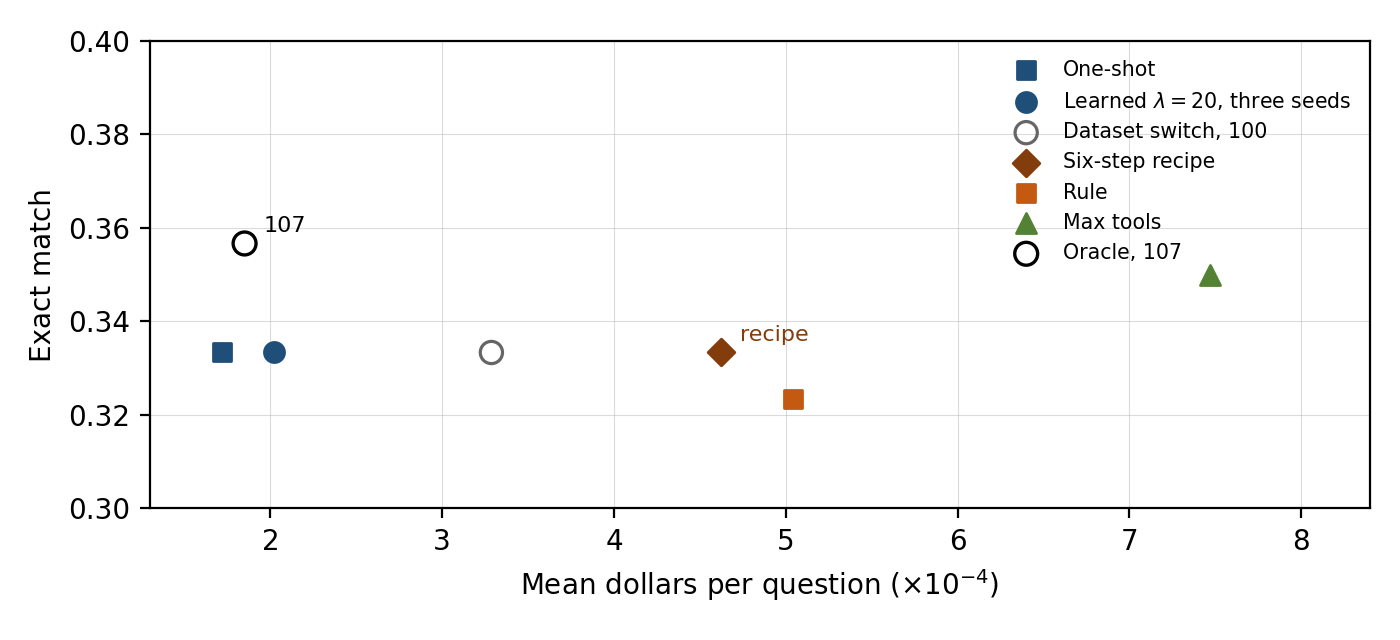
\includegraphics[width=0.92\textwidth]{paper_v4/figures/frontier.png}
\caption{Exact match against mean dollars per question on the 83{,}120-passage index. Squares are one-shot retrieval and the rule. The triangle is max tools. The diamond is the six-step recipe. The filled circle is the learned \(\lambda{=}20\) exam; seeds 42, 43, and 44 sit on the same point. Hollow circles are oracles: the dataset switch scores 100, and the oracle that may also use max tools scores 107. The oracle of one-shot retrieval and the six-step recipe is the one-shot point.}
\label{fig:frontier}
\end{figure*}

\subsection{Three Seeds Select One Recipe}
Table~\ref{tab:learned} is the \(\lambda{=}20\) exam. Seeds 42, 43, and 44 select epochs 17, 14, and 11, the first epoch that attains the best greedy reward on the 180 validation questions. The three exams match on every prediction, every action string, exact match, and reward. The action string is rewrite, rewrite, retrieve, stop on all 300 questions. Exact match is 100/300, HotpotQA 52/150 and Natural Questions 48/150, at \(2.02\times 10^{-4}\) dollars. The return under this preset, \(\lambda{=}20\) and \(\rho{=}0\), is 0.598 on each seed. That number is not comparable to the default-weight rewards in Table~\ref{tab:terms}. Measured latency, which is logged and not priced, is 3061 ms, 3000 ms, and 2956 ms.

\begin{table*}[t]
\centering
\small
\setlength{\tabcolsep}{8pt}
\begin{tabular*}{\textwidth}{@{\extracolsep{\fill}}lrrrrrr@{}}
\toprule
Seed & Epoch & HotpotQA & Natural Questions & Correct & Steps & \(\$\times 10^{-4}\) \\
\midrule
42 & 17 & 52/150 & 48/150 & 100/300 & 4 & 2.02 \\
43 & 14 & 52/150 & 48/150 & 100/300 & 4 & 2.02 \\
44 & 11 & 52/150 & 48/150 & 100/300 & 4 & 2.02 \\
\bottomrule
\end{tabular*}
\caption{The three \(\lambda{=}20\) exams. Each seed emits one action string, rewrite then rewrite then retrieve then stop. The rows tie on every reported value except the selected epoch, so no cell is marked as best. One-shot retrieval on the same index scores 100/300 at \(1.72\times 10^{-4}\) dollars. We report the three rows, not a mean.}
\label{tab:learned}
\end{table*}

Against one-shot retrieval the recipe agrees on 179 of 300 predictions. Of the 121 disagreements, 22 become correct, 22 become incorrect, 1 stays correct under a different string, and 76 stay wrong. The repairs and the breaks are HotpotQA \(+5\) and \(-13\), Natural Questions \(+17\) and \(-9\). The union is 122/300. Both policies are right on 78 questions, so \(78+22+22=122\).

That union is not the ceiling in Figure~\ref{fig:frontier}. The ceiling keeps the cheapest correct trajectory among one-shot retrieval, the six-step recipe, and max tools. The six-step recipe adds no new correct question, and max tools adds 7, so the ceiling is \(100+7=107\). The learned string is a different set of 100 correct questions. It is not one of the three trajectories in that oracle, and putting it in the oracle would be a different comparison from the one the figure reports. The average exact match does not move. The questions do.

The recipe never branches on the retrieval score. We count a seed only when the second action is sometimes rewrite and sometimes retrieve, at least 15 times each, and one threshold on the mean score matches at least 250 of those questions. Here the first action is already rewrite, so the second action still sees a mean score of 0 and no passages. That action is rewrite on all 300 questions, on all three seeds. Retrieve is never the second action. The count is 0 of 3.

Verify is not what moves the 44 answers. The learned recipe never calls it. The six-step recipe calls it twice on every question and still emits the same 300 answers as one-shot retrieval.

\subsection{Diagnostics}
An earlier observation passed the mean BM25 score through \(\tanh(\mathrm{score}/5)\). Top-1 scores on this corpus run from about 26 to 122, so that feature was 1.0 on all 300 questions and a policy could not branch on it. Standardizing the score makes a branch expressible. The three seeds do not use it. The first action is chosen before any score exists, and the selected string spends both rewrites before the first retrieve. The earlier saturated feature is the reason the branch had to be defined, not a second result.

\section{Limitations}
There are three limits on what these results support.

First, the controller never reads passage text. This is a study of the reward and of credit assignment in a small policy, not a fine-tune of the generator. The first action is the same on every question, because the observation before retrieval does not contain the question. The selected recipe rewrites twice before it retrieves, so the second action is still blind to the retrieval score. Adaptivity that depends on a score can start only after a retrieve.

Second, the three seeds are \(\lambda{=}20\) with the action charge off. They are three values of one setting. They are not a sweep of \(\lambda\), and they are not a standard deviation. The frozen rows in Table~\ref{tab:frozen} are one pass each, at temperature 0.

Third, the verifier and the reranker are lexical, and the price card is a scale for a local model. A neural verifier, a dense retriever, or a generator-sized policy could move the 7-answer gap and the dollar weight at which extra tools stop paying. That comparison was not run. A question-only classifier in the style of Adaptive-RAG, trained on the 500 training questions to choose one-shot retrieval or the rewrite-first recipe, is also not in the tables. Scoring both recipes on those 500 questions needs the generator, and that pass was not run. Adaptive-RAG, Self-RAG, CRAG, Search-R1, and GRASP remain Table~\ref{tab:related}.

\section{Conclusion}
On one index, extra tools buy five exact-match answers and lose reward. Max tools scores 105/300 against 100/300 for one-shot retrieval, and the reward falls from 0.581 to 0.503 because the action charge rises by more than the quality terms.

The per-question ceiling among the trajectories we logged is 107/300, at nearly the one-shot price, because the oracle pays for max tools only on the 7 answers it repairs. A frozen six-step recipe does not add a question. Three seeds of the learned policy select one four-step recipe, score 100/300, and disagree with one-shot retrieval on 44 questions. The branch on retrieval strength appears in 0 of 3 seeds, because that recipe rewrites before it ever sees a score.

A next controller has to read the question, or the passages, before it spends a rewrite. Three changes would test that. A neural verifier could replace the lexical check that currently changes no answer. A policy that reads the passage text could choose the second action from the evidence, not from a score of 0. GRPO, which compares several rollouts of the same question, is a closer trainer to GRASP than the one-sample REINFORCE update used here \cite{shao2024deepseekmath,gandhi2026grasp}. None of the three was run.

\section*{AI Use}
A language model was used to revise sentences and to check bibliography entries against paper abstracts. An image model drafted Figure~\ref{fig:pipeline}; the experimental plots were drawn from the logged numbers. No model output is reported as a measurement.

\section*{Ethical Statement}
Pricing a tool can refuse a search that would have changed the answer, and the user is not told. Fixed recipes score 97 to 105 out of 300, and an oracle that may use max tools reaches 107 near the one-shot price. The learned recipe and one-shot retrieval each score 100 and disagree on 44 questions. The abstention bonus does not fire on this corpus, and the selected checkpoints never call the verifier. The dollars are a scale for a local 3B model, not a bill a person pays. The questions and passages are public benchmarks with no human subjects, and the checkpoints are not a serving policy.

\FloatBarrier
\InputIfFileExists{included-bib.tex}{}{\begin{thebibliography}{36}
\providecommand{\natexlab}[1]{#1}

\bibitem[{Asai et~al.(2024)Asai, Wu, Wang, Sil, and Hajishirzi}]{asai2024selfrag}
Asai, A.; Wu, Z.; Wang, Y.; Sil, A.; and Hajishirzi, H. 2024.
\newblock Self-{RAG}: Learning to Retrieve, Generate, and Critique through Self-Reflection.
\newblock In \emph{International Conference on Learning Representations}.

\bibitem[{Borgeaud et~al.(2021)Borgeaud, Mensch, Hoffmann, Cai, Rutherford, Millican, van den Driessche, Lespiau, Damoc, Clark, de Las Casas, Guy, Menick, Ring, Hennigan, Huang, Maggiore, Jones, Cassirer, Brock, Paganini, Irving, Vinyals, Osindero, Simonyan, Rae, Elsen, and Sifre}]{borgeaud2022retro}
Borgeaud, S.; Mensch, A.; Hoffmann, J.; Cai, T.; Rutherford, E.; Millican, K.; van den Driessche, G.; Lespiau, J.-B.; Damoc, B.; Clark, A.; de Las Casas, D.; Guy, A.; Menick, J.; Ring, R.; Hennigan, T.; Huang, S.; Maggiore, L.; Jones, C.; Cassirer, A.; Brock, A.; Paganini, M.; Irving, G.; Vinyals, O.; Osindero, S.; Simonyan, K.; Rae, J.~W.; Elsen, E.; and Sifre, L. 2021.
\newblock Improving Language Models by Retrieving from Trillions of Tokens.
\newblock arXiv:2112.04426.

\bibitem[{Chen et~al.(2023)Chen, Zaharia, and Zou}]{chen2023frugalgpt}
Chen, L.; Zaharia, M.; and Zou, J. 2023.
\newblock {FrugalGPT}: How to Use Large Language Models While Reducing Cost and Improving Performance.
\newblock arXiv:2305.05176.

\bibitem[{Chen et~al.(2025)Chen, Sun, Li, Sun, Zhou, Zhu, Wang, Pan, Zhang, Chen, Yang, Zhou, and Chen}]{chen2025research}
Chen, M.; Sun, L.; Li, T.; Sun, H.; Zhou, Y.; Zhu, C.; Wang, H.; Pan, J.~Z.; Zhang, W.; Chen, H.; Yang, F.; Zhou, Z.; and Chen, W. 2025.
\newblock {ReSearch}: Learning to Reason with Search for {LLMs} via Reinforcement Learning.
\newblock arXiv:2503.19470.

\bibitem[{Gandhi et~al.(2026)Gandhi, Lee, Todmal, Dernoncourt, Rossi, Wang, and Lan}]{gandhi2026grasp}
Gandhi, V.; Lee, J.; Todmal, S.; Dernoncourt, F.; Rossi, R.~A.; Wang, Z.; and Lan, A. 2026.
\newblock {GRASP}: Granularity-Aware Search Policy for Agentic {RAG}.
\newblock arXiv:2607.10463.

\bibitem[{Gao et~al.(2022)Gao, Dai, Pasupat, Chen, Chaganty, Fan, Zhao, Lao, Lee, Juan, and Guu}]{gao2023rarr}
Gao, L.; Dai, Z.; Pasupat, P.; Chen, A.; Chaganty, A.~T.; Fan, Y.; Zhao, V.~Y.; Lao, N.; Lee, H.; Juan, D.-C.; and Guu, K. 2022.
\newblock {RARR}: Researching and Revising What Language Models Say, Using Language Models.
\newblock arXiv:2210.08726.

\bibitem[{Gao et~al.(2022)Gao, Ma, Lin, and Callan}]{gao2023hyde}
Gao, L.; Ma, X.; Lin, J.; and Callan, J. 2022.
\newblock Precise Zero-Shot Dense Retrieval without Relevance Labels.
\newblock arXiv:2212.10496.

\bibitem[{Gao et~al.(2022)Gao, Ma, Lin, and Callan}]{gao2022tevatron}
Gao, L.; Ma, X.; Lin, J.; and Callan, J. 2022.
\newblock Tevatron: An Efficient and Flexible Toolkit for Dense Retrieval.
\newblock arXiv:2203.05765.

\bibitem[{Guu et~al.(2020)Guu, Lee, Tung, Pasupat, and Chang}]{guu2020realm}
Guu, K.; Lee, K.; Tung, Z.; Pasupat, P.; and Chang, M.-W. 2020.
\newblock {REALM}: Retrieval-Augmented Language Model Pre-Training.
\newblock In \emph{Proceedings of the 37th International Conference on Machine Learning}, 3929--3938.

\bibitem[{Honovich et~al.(2022)Honovich, Aharoni, Herzig, Taitelbaum, Kukliansy, Cohen, Scialom, Szpektor, Hassidim, and Matias}]{honovich2022true}
Honovich, O.; Aharoni, R.; Herzig, J.; Taitelbaum, H.; Kukliansy, D.; Cohen, V.; Scialom, T.; Szpektor, I.; Hassidim, A.; and Matias, Y. 2022.
\newblock {TRUE}: Re-evaluating Factual Consistency Evaluation.
\newblock arXiv:2204.04991.

\bibitem[{Izacard and Grave(2020)}]{izacard2021fid}
Izacard, G.; and Grave, E. 2020.
\newblock Leveraging Passage Retrieval with Generative Models for Open Domain Question Answering.
\newblock arXiv:2007.01282.

\bibitem[{Izacard et~al.(2022)Izacard, Lewis, Lomeli, Hosseini, Petroni, Schick, Dwivedi-Yu, Joulin, Riedel, and Grave}]{izacard2023atlas}
Izacard, G.; Lewis, P.; Lomeli, M.; Hosseini, L.; Petroni, F.; Schick, T.; Dwivedi-Yu, J.; Joulin, A.; Riedel, S.; and Grave, E. 2022.
\newblock Atlas: Few-shot Learning with Retrieval Augmented Language Models.
\newblock arXiv:2208.03299.

\bibitem[{Jeong et~al.(2024)Jeong, Baek, Cho, Hwang, and Park}]{jeong2024adaptive}
Jeong, S.; Baek, J.; Cho, S.; Hwang, S.~J.; and Park, J.~C. 2024.
\newblock Adaptive-{RAG}: Learning to Adapt Retrieval-Augmented Large Language Models through Question Complexity.
\newblock In \emph{Proceedings of the 2024 Conference of the North American Chapter of the Association for Computational Linguistics: Human Language Technologies}, 7036--7050.

\bibitem[{Jiang et~al.(2023)Jiang, Xu, Gao, Sun, Liu, Dwivedi-Yu, Yang, Callan, and Neubig}]{jiang2023flare}
Jiang, Z.; Xu, F.~F.; Gao, L.; Sun, Z.; Liu, Q.; Dwivedi-Yu, J.; Yang, Y.; Callan, J.; and Neubig, G. 2023.
\newblock Active Retrieval Augmented Generation.
\newblock arXiv:2305.06983.

\bibitem[{Jin et~al.(2025)Jin, Zeng, Yue, Yoon, Arik, Wang, Zamani, and Han}]{jin2025searchr1}
Jin, B.; Zeng, H.; Yue, Z.; Yoon, J.; Arik, S.; Wang, D.; Zamani, H.; and Han, J. 2025.
\newblock Search-R1: Training {LLMs} to Reason and Leverage Search Engines with Reinforcement Learning.
\newblock arXiv:2503.09516.

\bibitem[{Karpukhin et~al.(2020)Karpukhin, O{\u{g}}uz, Min, Lewis, Wu, Edunov, Chen, and Yih}]{karpukhin2020dpr}
Karpukhin, V.; O{\u{g}}uz, B.; Min, S.; Lewis, P.; Wu, L.; Edunov, S.; Chen, D.; and Yih, W.-t. 2020.
\newblock Dense Passage Retrieval for Open-Domain Question Answering.
\newblock In \emph{Proceedings of the 2020 Conference on Empirical Methods in Natural Language Processing}, 6769--6781.

\bibitem[{Kwiatkowski et~al.(2019)Kwiatkowski, Palomaki, Redfield, Collins, Parikh, Alberti, Epstein, Polosukhin, Devlin, Lee, Toutanova, Jones, Kelcey, Chang, Dai, Uszkoreit, Le, and Petrov}]{kwiatkowski2019nq}
Kwiatkowski, T.; Palomaki, J.; Redfield, O.; Collins, M.; Parikh, A.; Alberti, C.; Epstein, D.; Polosukhin, I.; Devlin, J.; Lee, K.; Toutanova, K.; Jones, L.; Kelcey, M.; Chang, M.-W.; Dai, A.~M.; Uszkoreit, J.; Le, Q.; and Petrov, S. 2019.
\newblock Natural Questions: A Benchmark for Question Answering Research.
\newblock \emph{Transactions of the Association for Computational Linguistics}, 7: 452--466.

\bibitem[{Lewis et~al.(2020)Lewis, Perez, Piktus, Petroni, Karpukhin, Goyal, K{\"u}ttler, Lewis, Yih, Rockt{\"a}schel, Riedel, and Kiela}]{lewis2020rag}
Lewis, P.; Perez, E.; Piktus, A.; Petroni, F.; Karpukhin, V.; Goyal, N.; K{\"u}ttler, H.; Lewis, M.; Yih, W.-t.; Rockt{\"a}schel, T.; Riedel, S.; and Kiela, D. 2020.
\newblock Retrieval-Augmented Generation for Knowledge-Intensive {NLP} Tasks.
\newblock In \emph{Advances in Neural Information Processing Systems}, volume~33, 9459--9474.

\bibitem[{Ma et~al.(2023)Ma, Gong, He, Zhao, and Duan}]{ma2023rewrite}
Ma, X.; Gong, Y.; He, P.; Zhao, H.; and Duan, N. 2023.
\newblock Query Rewriting for Retrieval-Augmented Large Language Models.
\newblock arXiv:2305.14283.

\bibitem[{Nogueira and Cho(2019)}]{nogueira2019monobert}
Nogueira, R.; and Cho, K. 2019.
\newblock Passage Re-ranking with {BERT}.
\newblock arXiv:1901.04085.

\bibitem[{Ong et~al.(2024)Ong, Almahairi, Wu, Chiang, Wu, Gonzalez, Kadous, and Stoica}]{ong2024routellm}
Ong, I.; Almahairi, A.; Wu, V.; Chiang, W.-L.; Wu, T.; Gonzalez, J.~E.; Kadous, M.~W.; and Stoica, I. 2024.
\newblock {RouteLLM}: Learning to Route {LLMs} with Preference Data.
\newblock arXiv:2406.18665.

\bibitem[{Press et~al.(2022)Press, Zhang, Min, Schmidt, Smith, and Lewis}]{press2023selfask}
Press, O.; Zhang, M.; Min, S.; Schmidt, L.; Smith, N.~A.; and Lewis, M. 2022.
\newblock Measuring and Narrowing the Compositionality Gap in Language Models.
\newblock arXiv:2210.03350.

\bibitem[{{Qwen Team}(2024)}]{qwen2024}
{Qwen Team}. 2024.
\newblock Qwen2.5 Technical Report.
\newblock arXiv:2412.15115.

\bibitem[{Rajpurkar et~al.(2016)Rajpurkar, Zhang, Lopyrev, and Liang}]{rajpurkar2016squad}
Rajpurkar, P.; Zhang, J.; Lopyrev, K.; and Liang, P. 2016.
\newblock {SQuAD}: 100{,}000+ Questions for Machine Comprehension of Text.
\newblock In \emph{Proceedings of the 2016 Conference on Empirical Methods in Natural Language Processing}.

\bibitem[{Robertson and Zaragoza(2009)}]{robertson2009bm25}
Robertson, S.; and Zaragoza, H. 2009.
\newblock The Probabilistic Relevance Framework: {BM25} and Beyond.
\newblock \emph{Foundations and Trends in Information Retrieval}, 3(4): 333--389.

\bibitem[{Schick et~al.(2023)Schick, Dwivedi-Yu, Dess{\`i}, Raileanu, Lomeli, Zettlemoyer, Cancedda, and Scialom}]{schick2023toolformer}
Schick, T.; Dwivedi-Yu, J.; Dess{\`i}, R.; Raileanu, R.; Lomeli, M.; Zettlemoyer, L.; Cancedda, N.; and Scialom, T. 2023.
\newblock Toolformer: Language Models Can Teach Themselves to Use Tools.
\newblock arXiv:2302.04761.

\bibitem[{Schulman et~al.(2017)Schulman, Wolski, Dhariwal, Radford, and Klimov}]{schulman2017ppo}
Schulman, J.; Wolski, F.; Dhariwal, P.; Radford, A.; and Klimov, O. 2017.
\newblock Proximal Policy Optimization Algorithms.
\newblock arXiv:1707.06347.

\bibitem[{Shao et~al.(2024)Shao, Wang, Zhu, Xu, Song, Bi, Zhang, Zhang, Li, Wu, and Guo}]{shao2024deepseekmath}
Shao, Z.; Wang, P.; Zhu, Q.; Xu, R.; Song, J.; Bi, X.; Zhang, H.; Zhang, M.; Li, Y.~K.; Wu, Y.; and Guo, D. 2024.
\newblock {DeepSeekMath}: Pushing the Limits of Mathematical Reasoning in Open Language Models.
\newblock arXiv:2402.03300.

\bibitem[{Song et~al.(2025)Song, Jiang, Min, Chen, Chen, Zhao, Fang, and Wen}]{song2025r1searcher}
Song, H.; Jiang, J.; Min, Y.; Chen, J.; Chen, Z.; Zhao, W.~X.; Fang, L.; and Wen, J.-R. 2025.
\newblock R1-Searcher: Incentivizing the Search Capability in {LLMs} via Reinforcement Learning.
\newblock arXiv:2503.05592.

\bibitem[{Su et~al.(2024)Su, Tang, Ai, Wu, and Liu}]{su2024dragin}
Su, W.; Tang, Y.; Ai, Q.; Wu, Z.; and Liu, Y. 2024.
\newblock {DRAGIN}: Dynamic Retrieval Augmented Generation based on the Information Needs of Large Language Models.
\newblock arXiv:2403.10081.

\bibitem[{Sun et~al.(2023)Sun, Yan, Ma, Wang, Ren, Chen, Yin, and Ren}]{sun2023rankgpt}
Sun, W.; Yan, L.; Ma, X.; Wang, S.; Ren, P.; Chen, Z.; Yin, D.; and Ren, Z. 2023.
\newblock Is {ChatGPT} Good at Search? Investigating Large Language Models as Re-Ranking Agents.
\newblock arXiv:2304.09542.

\bibitem[{Trivedi et~al.(2022)Trivedi, Balasubramanian, Khot, and Sabharwal}]{trivedi2023ircot}
Trivedi, H.; Balasubramanian, N.; Khot, T.; and Sabharwal, A. 2022.
\newblock Interleaving Retrieval with Chain-of-Thought Reasoning for Knowledge-Intensive Multi-Step Questions.
\newblock arXiv:2212.10509.

\bibitem[{Williams(1992)}]{williams1992reinforce}
Williams, R.~J. 1992.
\newblock Simple Statistical Gradient-Following Algorithms for Connectionist Reinforcement Learning.
\newblock \emph{Machine Learning}, 8(3--4): 229--256.

\bibitem[{Yan et~al.(2024)Yan, Gu, Zhu, and Ling}]{yan2024crag}
Yan, S.-Q.; Gu, J.-C.; Zhu, Y.; and Ling, Z.-H. 2024.
\newblock Corrective Retrieval Augmented Generation.
\newblock arXiv:2401.15884.

\bibitem[{Yang et~al.(2018)Yang, Qi, Zhang, Bengio, Cohen, Salakhutdinov, and Manning}]{yang2018hotpotqa}
Yang, Z.; Qi, P.; Zhang, S.; Bengio, Y.; Cohen, W.~W.; Salakhutdinov, R.; and Manning, C.~D. 2018.
\newblock {HotpotQA}: A Dataset for Diverse, Explainable Multi-hop Question Answering.
\newblock In \emph{Proceedings of the 2018 Conference on Empirical Methods in Natural Language Processing}, 2369--2380.

\bibitem[{Yao et~al.(2023)Yao, Zhao, Yu, Du, Shafran, Narasimhan, and Cao}]{yao2023react}
Yao, S.; Zhao, J.; Yu, D.; Du, N.; Shafran, I.; Narasimhan, K.; and Cao, Y. 2023.
\newblock {ReAct}: Synergizing Reasoning and Acting in Language Models.
\newblock In \emph{International Conference on Learning Representations}.

\end{thebibliography}
}

\end{document}
